

EcoDrive models various forces as functions of instant fuel consumption and produces fuel consumption profile as output. 
Different from Existing vehicle dynamics models \cite{koprubasi2008modeling},  
we only use parameters available from OBD instead of assuming 
the engine parameters are known in advance. 
We consider several factors that affect car fuel
consumption, e.g., engine torque, 
drivetrain loss, wind resistance and grade resistance.   
The vehicle force can be modeled as follows. 

\begin{equation}
F = F_p - F_l - F_g - F_w.
\end{equation}

where $F_p$ refers to the propulsion caused by car engine, 
$F_l$ refers to the drivetrain loss caused by transmission and various gears 
connecting engine and wheels,
$F_w$ refers to the wind resistance,
$F_g$ refers to the grade resistance. 
Since we are only interested in fuel consumption on acceleration
and cruise, we exclude the forces caused by brake. 

We model the forces in the following steps.  
First, we use RPM and vehicular speed to model gear ratio and use 
AFR to model engine torque. 
Second, the drivetrain loss and wind resistance is modeled as
the counterforce of propulsion when the car is driven in constant speeds. 
Finally, we use driving data extracted from flat road to 
train the parameters of our propulsion and 
loss models, and then use the propulsion model
to model grade resistance.




\begin{figure*}[t]
\begin{center}
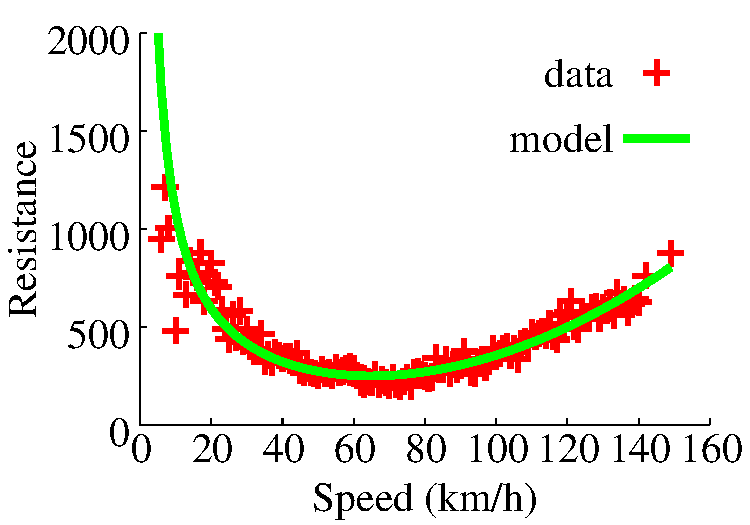
\includegraphics[width=1.8in,angle=0]{Figs/EcoDrive/lei_loss.pdf}
\hspace{-0.0cm}
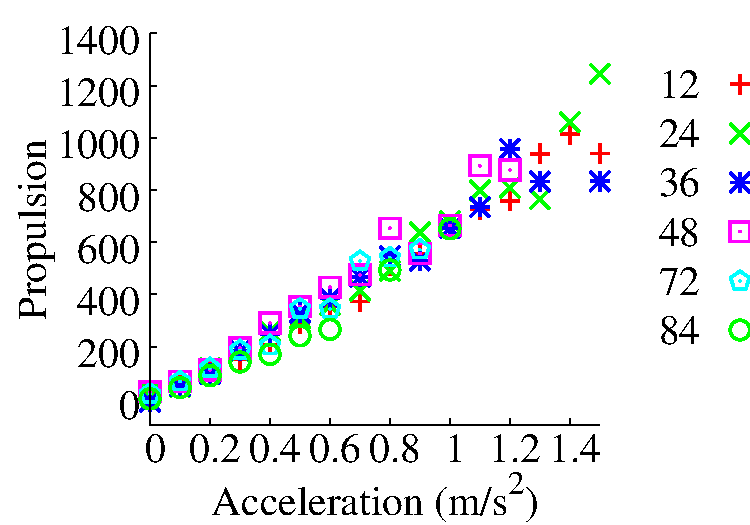
\includegraphics[width=1.8in,angle=0]{Figs/EcoDrive/lei_torque.pdf}
\hspace{-0.0cm}
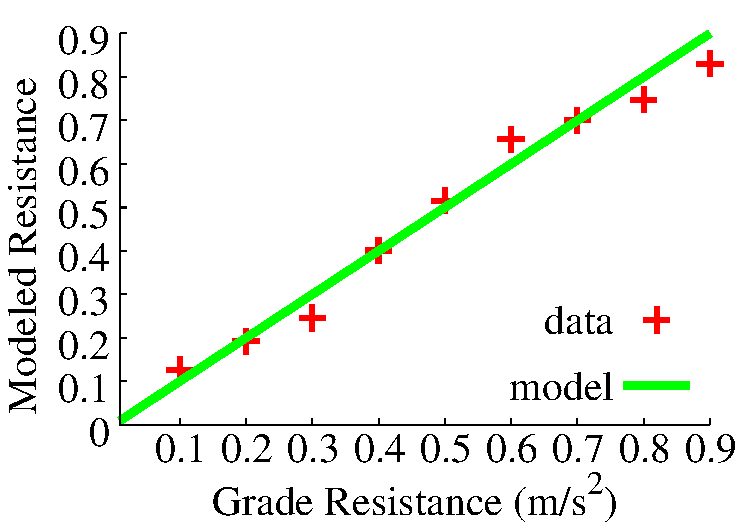
\includegraphics[width=1.8in,angle=0]{Figs/EcoDrive/lei_slope.pdf}
\hspace{-0.0cm}
\vspace{-0.2cm}
\caption{Vehicle Dynamics Modeling. The Figs/EcoDrive are about drivetrain loss and wind resistance under each speed (left), 
relation between acceleration and propulsion (minus wind resistance and drivetrain loss) under each speed (middle), 
modeled grade resistance with groundtruth (right).}
\vspace{-0.8cm}
\label{modeling}
\end{center}
\end{figure*}

\subsection{Propulsion Modeling}


The propulsion (or output torque) of vehicle is closely related
to transmission gear ratios and engine torque \cite{vong2006prediction, giannelli2005heavy}. 
The propulsion produced by vehicle engine
can be represented by

\begin{equation}
 F_p = a_p * \tau_e * R_G.
\end{equation}

where $\tau_e$ refers to the engine torque, 
$R_G$ refers to transmission gear ratio
and $a_p$ is the coefficient used for unit conversion. 


\subsubsection{Gear Ratio Modeling}

Modern vehicles are usually using automatic transmission and 
freeing the driver from shifting gears manually. 
There are mainly two types of transmissions, 
Step Automatic Transmission (SAT) and Continuously Variable Transmission (CVT). 
SAT uses discrete transmission gear ratios while CVT has an
infinite number of effective transmission gear ratios. 
Since different transmission types show different
properties of gear ratio changes over different speeds, 
we use gear ratio changes to identify different
vehicle transmission types. 
We estimate gear ratios by using RPM and speeds 
when the car is driving in constant speeds. 



In a SAT vehicle, $R_G$ are discrete values.
  
\begin{equation}
   R_G = R_i = \frac{RPM}{v}  \hspace{1cm} i = 1,...,n
 \end{equation}

where $v$ represents the vehicular speed 
and $n$ is the number of gears of a transmission, 
e.g., $n=4$ for a 4-speed transmission. 

In a CVT vehicle, $R_G$ changes continuously over time and always
approach the optimal $RPM$. 

\begin{equation}
   R_G =
   \begin{cases}
   \frac{RPM_a}{v}     &  \mbox{if} \hspace{0.2cm} v < v_T, \\
   R_b   &  \mbox{if} \hspace{0.2cm} v \geq v_T.
   \end{cases}
  \end{equation}

where $RPM_a$ is the optimal $RPM$ of a given engine, 
and $v_T$ is the speed threshold. 
If the vehicular speed is lower than $v_T$, 
the engine $RPM$ converges to a constant value $RPM_a$ under
different speeds. 
If the vehicular speed is higher than or equal to $v_T$, 
the gear ratio is a constant value $R_b$. 


\subsubsection{Engine Torque Modeling}


\nop{
\begin{figure}[t]
\begin{center}
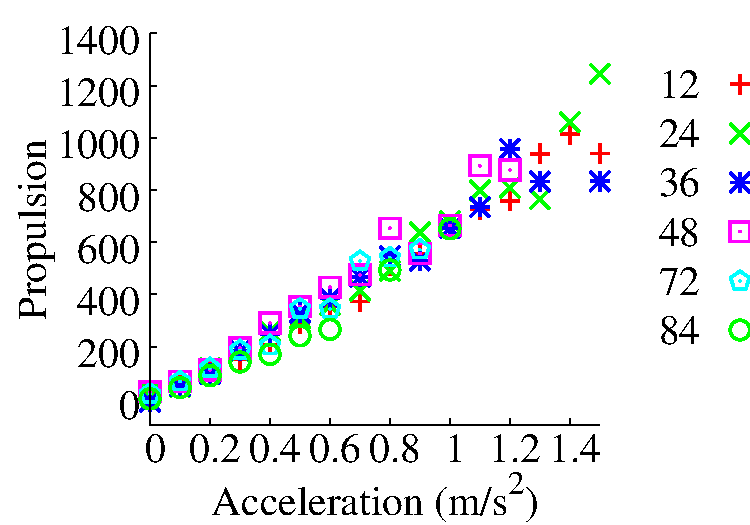
\includegraphics[width=3.0in,angle=0]{Figs/EcoDrive/lei_torque.pdf}
\vspace{-1.0cm}
\caption{Propulsion (output torque) under different speeds (km/h)
and accelerations.}
\vspace{-0.3cm}
\label{speed_propulsion}
\end{center}
\end{figure}
}

Engine torque is produced by the explosion of air and fuel, 
therefore, we can use AFR to model engine torque. 

\begin{equation}
\tau_e = AFR^{f(v)}.
\end{equation}


where $f(v)$ is a parameter function that is monotonically increasing
with vehicular speed. Based on our empirical observation, 
it starts from 0.3 at speed 0 and converges to 1 when the speed
is larger than $20km/h$. 

Therefore, the propulsion of a car on the wheel can be written as 

\begin{equation}
 F_p = a_p * \tau_e * R_G = a_p \frac{AFR^{f(v)} * RPM}{v}.
\end{equation}



\subsection{Drivetrain Loss and Wind Resistance Modeling}

\nop{
\begin{figure}[t]
\begin{center}
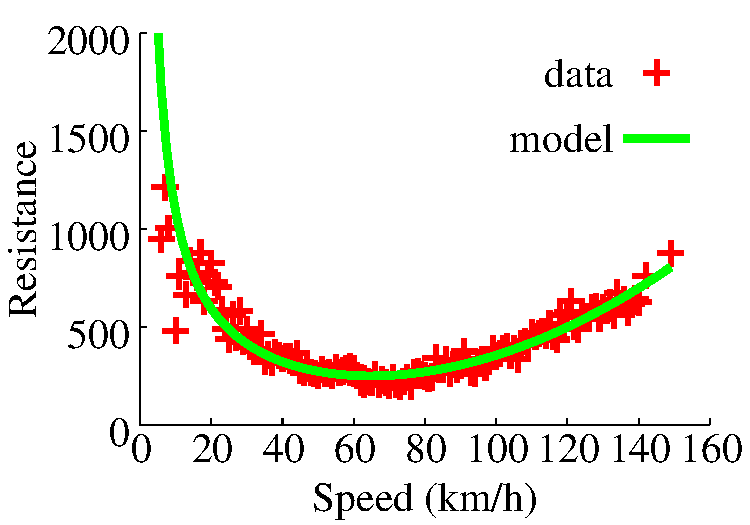
\includegraphics[width=2.4in,angle=0]{Figs/EcoDrive/lei_loss.pdf}
\vspace{-0.3cm}
\caption{Drivetrain loss and wind resistance under different speeds.}
\vspace{-0.3cm}
\label{speed_loss}
\end{center}
\end{figure}
}

Instead of modeling each loss individually, we model all the power losses
as a whole. 
There are mainly two power losses in automotive systems, 
drivetrain loss and wind resistance. 
Drivetrain loss consists of transmission loss and other mechanical system losses.  
Transmission connects car engine and wheels by various gears and
power loss occurs when transmit the power from engine to wheels. 
We model drivetrain loss in the following form.

\begin{equation}
F_l = \frac{a_l}{v} + b_l * v + c_l. 
\end{equation}

where $v$ is the vehicular speed and the rest are coefficients. 
The drivetrain loss drops to minimum when the car is driving
in moderate speed. 


The force from the air drag \cite{andersson2012online} 
can be represented by following equation,

\begin{equation}
 F_w = 0.5 * \rho_a * c_d * A_a * v^2 = a_w * v^2.
\end{equation}

where $\rho_a$ is the air mass density, 
$c_d$ is the air drag coefficient and 
$A_a$ is the effective area of the vehicle. 
Since the effective area of vehicle is different
from vehicle to vehicle, 
we model air drag as a function of vehicle speed
with unknown coefficient $a_w$. 


After we put drivetrain loss and wind resistance together, 
the modeled loss and actual loss are shown in the Fig. \ref{modeling}. 
In low speed, the main loss comes from drivetrain loss due
to mechanical frictions. 
In high speed, the main loss comes from wind resistance due to air compression. 
After we have drivetrain loss and wind resistance, 
we use propulsion minus the loss ($F_p - F_l - F_w$) to model the relation
between acceleration and propulsion, as shown in the middle of Fig. \ref{modeling}. 
For accelerations, we use extra $MAF$ instead of raw $MAF$ readings from 
the OBD port. 
Raw $MAF$ minus the $MAF$ required to maintain a certain speed is
the extra $MAF$ for this speed. 

\subsection{Grade Resistance Modeling}


\nop{
\begin{figure}[t]
\begin{center}
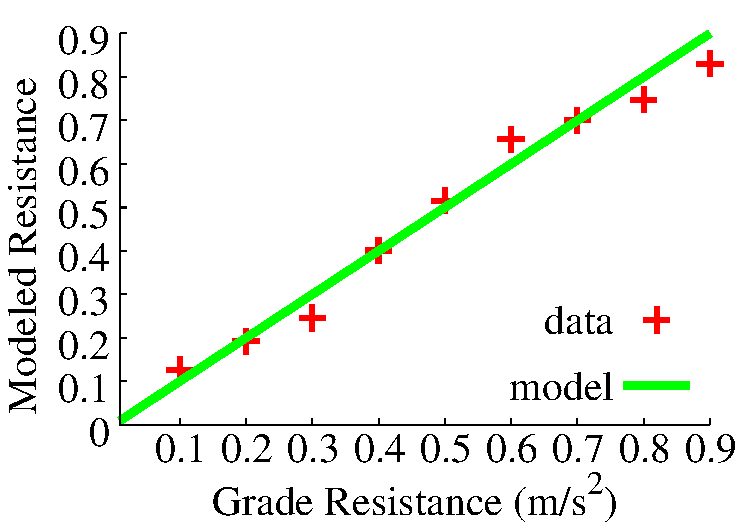
\includegraphics[width=2.5in,angle=0]{Figs/EcoDrive/lei_slope.pdf}
\vspace{-0.3cm}
\caption{Grade resistance.}
\vspace{-0.3cm}
\label{grade_resistance}
\end{center}
\end{figure}
}

Different road types, i.e., flat road, uphill and downhill, 
have significant different impacts on vehicle movements and
fuel consumptions. 
Similar to \cite{andersson2012online}, 
the grade resistance can be modeled as a combination
of forces caused by grade and rolling resistance.
\nop{
Since rolling resistance is a linear function of speed, 
so we combine it with wind resistance and focus on
grade resistance only. 
}
\begin{equation}
    F_r = mgc_r\cos{\theta}.
 \end{equation}
 
where $c_r$ is the grade resistance coefficient, 
$m$ is the vehicle mass, $g$ is the gravity of earth
, $\theta$ is the road grade and $v$ is vehicular speed.
The road elevation information is obtained from
National Elevation Dataset \cite{nationalelevation}. 
\nop{
The dataset provides fine-grained GPS elevation.
We compared the elevation dataset with Google Elevation
API \cite{googleelevation} on some routes,
and the results show that both datasets show similar accuracy. 
}




\subsection{AFR Profile}

Vehicle needs different air/fuel injection rate to achieve
different accelerations under different speeds. 
Based on the vehicle dynamics models we built in 
previous sections, we can build a fuel consumption profile. 
In this profile, we can lookup the AFR required to accelerate
a vehicle with an arbitrary acceleration under any speed. 
Let $AFR(v, a)$ denotes the air/fuel rate is required to 
accelerate the vehicle at acceleration $a$ when the vehicle
is driving at speed $v$. 
The profile can be represented as the following equation. 


\begin{equation}
AFR(v, a) = e^{\frac{log(a/R_G)}{f(v)}} + AFR_c(v)
\end{equation}


\begin{figure}[!htbp]
\begin{center}
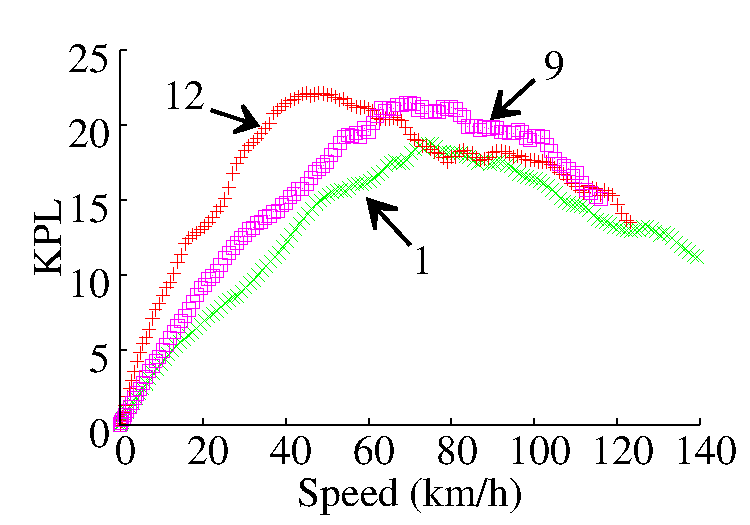
\includegraphics[width=3.0in,angle=0]{Figs/EcoDrive/speed_kpl.pdf}
\hspace{-0.4cm}
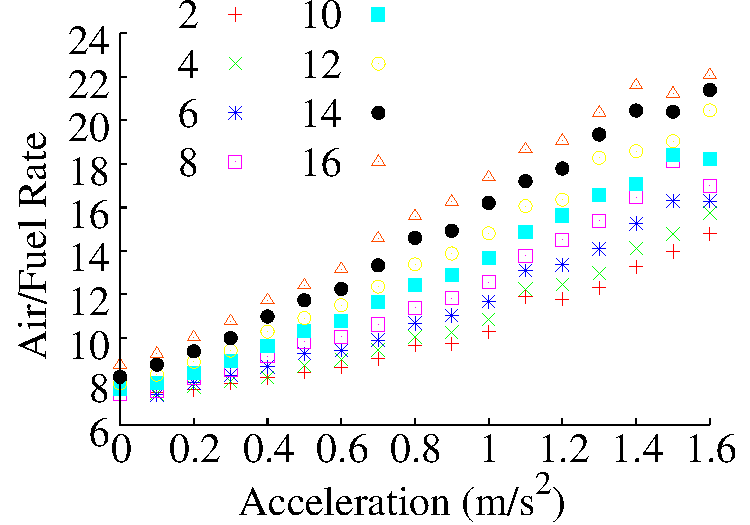
\includegraphics[width=3.0in,angle=0]{Figs/EcoDrive/acce_afr.pdf}
\hspace{-0.4cm}
\vspace{-0.3cm}
\caption{AFR profile.}
\vspace{-0.5cm}
\label{profile}
\end{center}
\end{figure}

An illustration of AFR profile of car 1 is shown in
the right subfigure of Fig. \ref{profile}. 
The profile provides the AFR required to accelerate the car
at a certain acceleration under a certain speed. 
We can infer a lookup table for each $AFR(v, a)$ based
on the profile. 
The left subfigure in Fig. \ref{profile} illustrates different
vehicles have different speed-KPL matching, 
which indicates AFR profile needs to be built
based on individual vehicles. 




 



